\documentclass[12pt]{article}                         
\pagestyle{plain}

\usepackage{amsmath}     % Enhanced math environments (e.g., align).
\usepackage{amsfonts}    % Math fonts (e.g., \mathfrak{}).
\usepackage{amstext}     % Text inside math mode (e.g., \text{where}).
\usepackage{amssymb}     % Extra math symbols (e.g., \mathbb{R}).
\usepackage{array}       % Advanced table/array column definitions.
\usepackage{circledtext} % Puts text inside a circle (e.g., \circledtext{A}).
\usepackage{comment}     % Include/exclude blocks of text.
\usepackage{enumerate}   % Customize itemized/numbered lists.
\usepackage{graphicx}    % Include images/graphics (\includegraphics).
\usepackage{latexsym}    % Access to basic LaTeX symbols.
\usepackage{multicol}    % Allows text columns on a page.
\usepackage{pgfplots}    % Create scientific plots from data (based on TikZ).
\usepackage{tabularx}    % Tables that stretch to page width.
\usepackage{tasks}       % Create multi-column lists.
\usepackage{textcomp}    % Provides many text symbols (e.g., \textcelsius).
\usepackage{tikz}        % Create vector graphics and diagrams.
\usepackage{xcolor}      % Define and use colors.
\usepackage{fancyhdr}
\usepackage{tcolorbox}
\usepackage{enumitem}

\usepackage[
  letterpaper,
  left=0.8in,
  right=0.8in,
  textheight=9.5in,
  bmargin=0.5in  % Adjust this value to push the footer down
]{geometry}
\pagestyle{fancy}
\fancyhf{} % Clear all header and footer fields
\fancyhead[L]{Your Name:} % Left header with name
\fancyhead[R]{Novemeber 18th 2025} % Right header with date
\renewcommand{\headrulewidth}{0.4pt} % Horizontal line below the header

\begin{document}

% Main title
\begin{center}
    \Large \textbf{Math 115E Activity 19} \\
    \vspace{0.2cm}
    \normalsize B4 Quiz Review
\end{center}
\vspace{-0.5cm}
\subsection*{Graphing Quadratic Functions}
\begin{minipage}[c]{0.60\textwidth}

\begin{enumerate}[label=\#\arabic*]
    \item Given the Function $f(x)=-5x^2 + 10x$
    \begin{enumerate}
        \item Find the x-intercepts:
        \\\\
        \item Find the y-intercepts:
        \\\\
        \item Find the Vertex:
        \\\\
        \item Sketch the Graph:
    \end{enumerate}
    \item Given the Function $g(x)=x^2+2x-3$
    \begin{enumerate}
        \item Find the x-intercepts:
        \\\\
        \item Find the y-intercepts:
        \\\\
        \item Find the Vertex
        \\\\
        \item Sketch the Graph:
    \end{enumerate}

    \item Given the Function $h(x)=(3-x)(1+x)$
    \begin{enumerate}
        \item Find the x-intercepts:
        \\\\
        \item Find the y-intercepts:
        \\\\
        \item Find the Vertex:
        \\\\
        \item Sketch the Graph:
    \end{enumerate}

\end{enumerate}
\end{minipage}
\hfill
\begin{minipage}[c]{0.40\textwidth}
\vspace{-1cm}
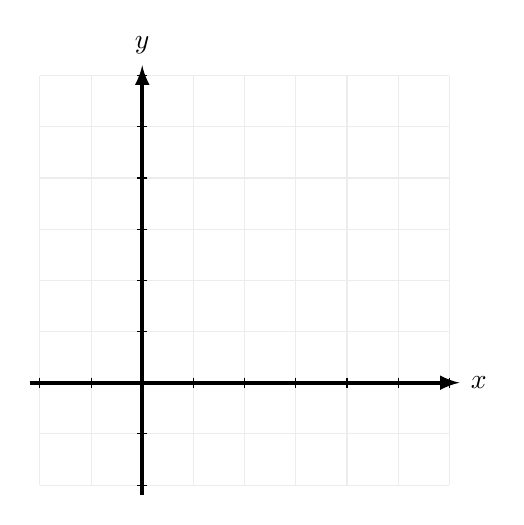
\begin{tikzpicture}
	[
		scale=0.65,
		vector style/.style={->, very thick}
	]
    \draw[gray!15,step=1cm] (-2,-2) grid (6,6);
    \draw[line width=0.5mm, -latex] (-2.2,0) -- (6.2,0) node[right] {$x$};
    \foreach \x in {-2,-1,1,2,3,4,5,6} \draw (\x,.1)--(\x,-.1) node[below] {};
    \draw[line width=0.5mm,  -latex] (0,-2.2) -- (0,6.2) node[above] {$y$};
    \foreach \y in {-2,-1,1,2,3,4,5,6} \draw (.1,\y)--(-.1,\y) node[left] {};
    %\draw[cyan,line width=2pt,latex-latex] plot[domain= 0:2, samples=100] (\x, {-5*(\x)^2 + 10*\x});
\end{tikzpicture}
\\\\\\
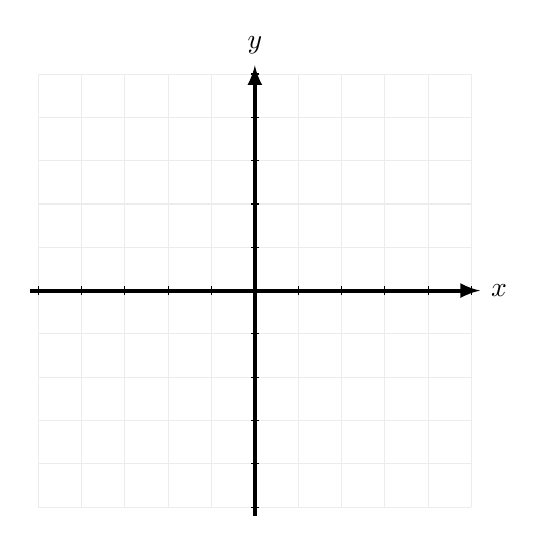
\begin{tikzpicture}
	[
		scale=0.55,
		vector style/.style={->, very thick}
	]
    \draw[gray!15,step=1cm] (-5,-5) grid (5,5);
        \draw[line width=0.5mm, -latex] (-5.2,0) -- (5.2,0) node[right] {$x$};
        \foreach \x in {-5,-4,-3,-2,-1,1,2,3,4,5} \draw (\x,.1)--(\x,-.1);
        \draw[line width=0.5mm,  -latex] (0,-5.2) -- (0,5.2) node[above] {$y$};
        \foreach \y in {-5,-4,-3,-2,-1,1,2,3,4,5} \draw (.1,\y)--(-.1,\y);
        %\draw[cyan,line width=2pt,latex-latex] plot[domain= -4:2, samples=100] (\x,{(\x)^2 + 2*\x - 3});
\end{tikzpicture}
\\\\\\
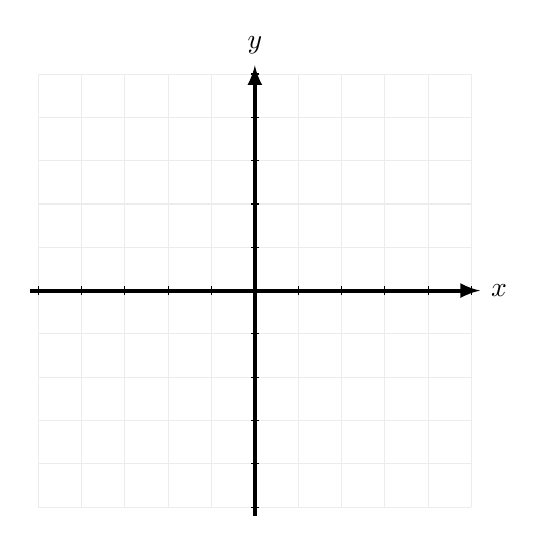
\begin{tikzpicture}
	[
		scale=0.55,
		vector style/.style={->, very thick}
	]
    \draw[gray!15,step=1cm] (-5,-5) grid (5,5);
        \draw[line width=0.5mm, -latex] (-5.2,0) -- (5.2,0) node[right] {$x$};
        \foreach \x in {-5,-4,-3,-2,-1,1,2,3,4,5} \draw (\x,.1)--(\x,-.1);
        \draw[line width=0.5mm,  -latex] (0,-5.2) -- (0,5.2) node[above] {$y$};
        \foreach \y in {-5,-4,-3,-2,-1,1,2,3,4,5} \draw (.1,\y)--(-.1,\y);
        %\draw[cyan,line width=2pt,latex-latex] plot[domain= -2:4, samples=100] (\x,{(3-\x)*(1+\x)});
    \end{tikzpicture}
\end{minipage}
\begin{minipage}[c]{0.60\textwidth}

\begin{enumerate}[label=\#\arabic*]
    \item Given the Function $k(x)= \displaystyle\frac{1}{2}x+2$
    \begin{enumerate}
        \item Find the x-intercepts:
        \\\\
        \item Find the y-intercepts:
        \\\\
        \item Find the Vertex:
        \\\\
        \item Sketch the Graph:
    \end{enumerate}

    \item Given the Function $j(x)=2x^2+2$
    \begin{enumerate}
        \item Find the x-intercepts:
        \\\\
        \item Find the y-intercepts:
        \\\\
        \item Find the Vertex:
        \\\\
        \item Sketch the Graph:
    \end{enumerate}

    \item Given the Function $p(x)=x^2-4x$
    \begin{enumerate}
        \item Find the x-intercepts:
        \\\\
        \item Find the y-intercepts:
        \\\\
        \item Find the Vertex:
        \\\\
        \item Sketch the Graph:
    \end{enumerate}

\end{enumerate}
\end{minipage}
\hfill
\begin{minipage}[c]{0.40\textwidth}

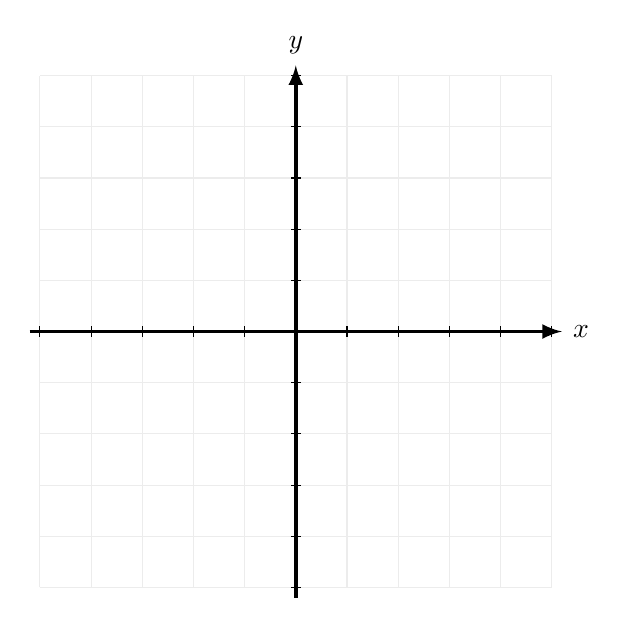
\begin{tikzpicture}
	[
		scale=0.65,
		vector style/.style={->, very thick}
	]
    \draw[gray!15,step=1cm] (-5,-5) grid (5,5);
        \draw[line width=0.5mm, -latex] (-5.2,0) -- (5.2,0) node[right] {$x$};
        \foreach \x in {-5,-4,-3,-2,-1,1,2,3,4,5} \draw (\x,.1)--(\x,-.1);
        \draw[line width=0.5mm,  -latex] (0,-5.2) -- (0,5.2) node[above] {$y$};
        \foreach \y in {-5,-4,-3,-2,-1,1,2,3,4,5} \draw (.1,\y)--(-.1,\y);
        %\draw[cyan,line width=2pt,latex-latex] plot[domain= -5:5, samples=100] (\x, {(1/2)*\x+2});
\end{tikzpicture}
\\\\\\
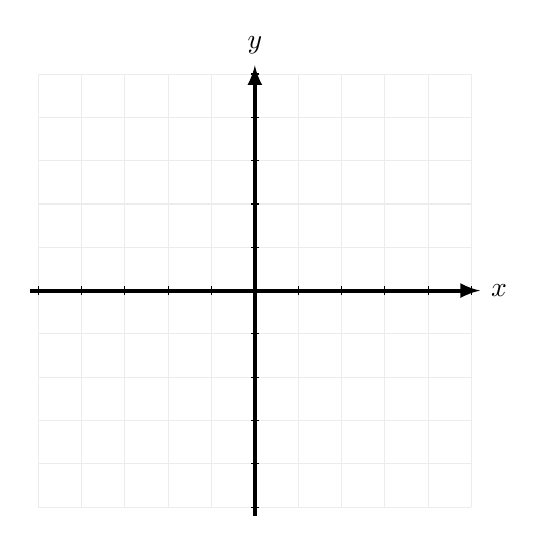
\begin{tikzpicture}
	[
		scale=0.55,
		vector style/.style={->, very thick}
	]
    \draw[gray!15,step=1cm] (-5,-5) grid (5,5);
        \draw[line width=0.5mm, -latex] (-5.2,0) -- (5.2,0) node[right] {$x$};
        \foreach \x in {-5,-4,-3,-2,-1,1,2,3,4,5} \draw (\x,.1)--(\x,-.1);
        \draw[line width=0.5mm,  -latex] (0,-5.2) -- (0,5.2) node[above] {$y$};
        \foreach \y in {-5,-4,-3,-2,-1,1,2,3,4,5} \draw (.1,\y)--(-.1,\y);
        %\draw[cyan,line width=2pt,latex-latex] plot[domain= -1.92:1.92, samples=100] (\x,{2*(\x)^2 - 2});
\end{tikzpicture}
\\\\\\
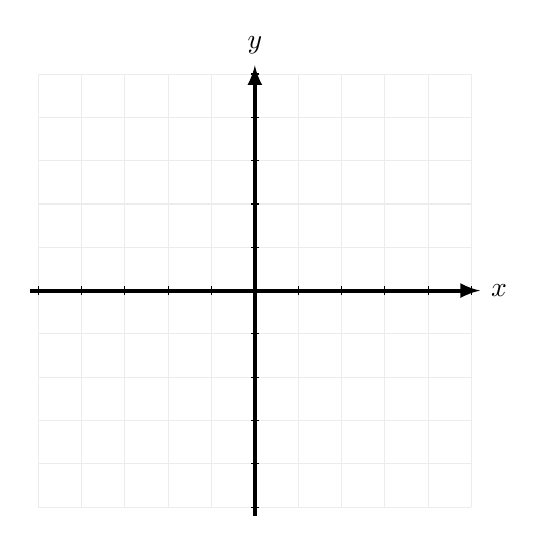
\begin{tikzpicture}
	[
		scale=0.55,
		vector style/.style={->, very thick}
	]
    \draw[gray!15,step=1cm] (-5,-5) grid (5,5);
        \draw[line width=0.5mm, -latex] (-5.2,0) -- (5.2,0) node[right] {$x$};
        \foreach \x in {-5,-4,-3,-2,-1,1,2,3,4,5} \draw (\x,.1)--(\x,-.1);
        \draw[line width=0.5mm,  -latex] (0,-5.2) -- (0,5.2) node[above] {$y$};
        \foreach \y in {-5,-4,-3,-2,-1,1,2,3,4,5} \draw (.1,\y)--(-.1,\y);
        %\draw[cyan,line width=2pt,latex-latex] plot[domain= -0.98:5, samples=100] (\x,{(\x)^2-4*\x});
    \end{tikzpicture}
\end{minipage}
\end{document}